\documentclass[11pt]{article}
\usepackage[utf8]{inputenc}
\usepackage[T1]{fontenc}
\usepackage{lmodern}
\usepackage{geometry}
\usepackage{tikz}
\usetikzlibrary{arrows.meta,shapes.geometric}

\geometry{paperwidth=11.4cm,paperheight=10.2cm,margin=0cm}
\pagestyle{empty}
\setlength{\parindent}{0pt}

\definecolor{ctxFill}{RGB}{238,242,245}
\definecolor{ctxLine}{RGB}{155,168,179}
\definecolor{ctxText}{RGB}{38,52,67}
\definecolor{exFill}{RGB}{220,233,247}
\definecolor{exLine}{RGB}{23,54,93}
\definecolor{prFill}{RGB}{200,240,236}
\definecolor{prLine}{RGB}{8,127,140}
\definecolor{prText}{RGB}{6,79,87}

\begin{document}
\noindent
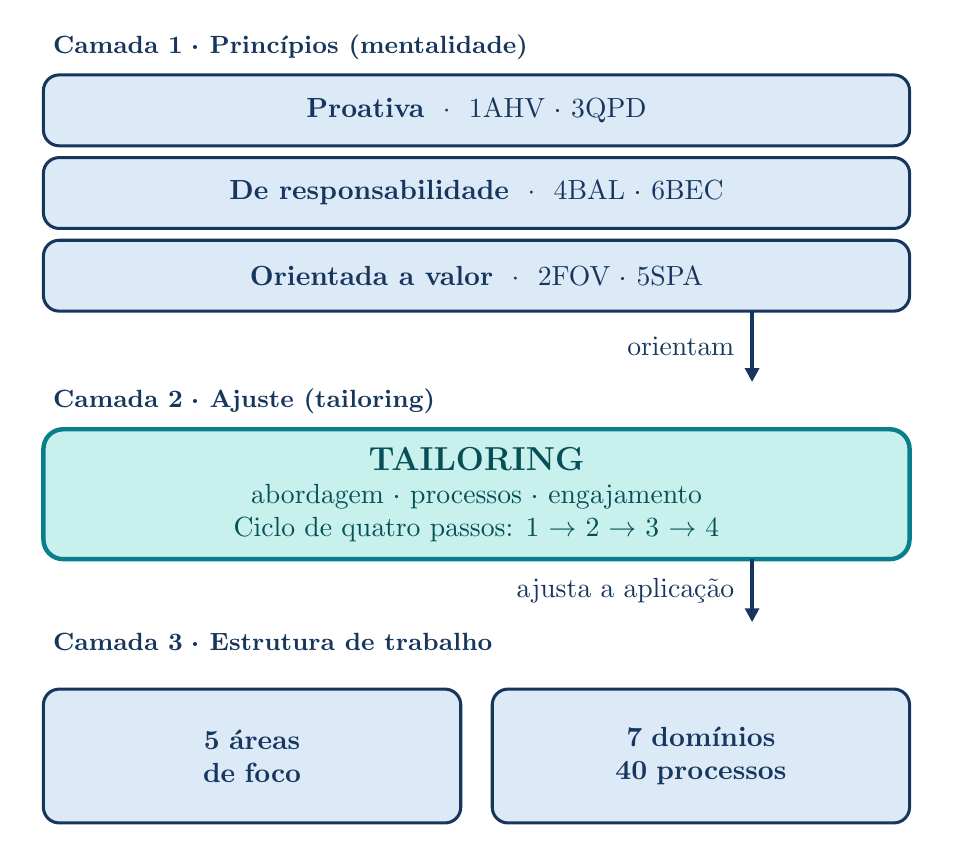
\begin{tikzpicture}[x=1cm,y=1cm,font=\small]
  \path[use as bounding box] (0,0) rectangle (11.4,10.2);
  \begin{scope}[xshift=0.2cm]
  \node[anchor=west,text=exLine,font=\small] at (0,9.95) {\textbf{Camada 1 · Princípios (mentalidade)}};
  \draw[fill=exFill,draw=exLine,line width=1.1pt,rounded corners=0.2cm] (0,8.7) rectangle (11,9.6);
  \node[text=exLine,font=\normalsize] at (5.5,9.149999999999999) {\textbf{Proativa} \ $\cdot$ \ 1AHV · 3QPD};
  \draw[fill=exFill,draw=exLine,line width=1.1pt,rounded corners=0.2cm] (0,7.6499999999999995) rectangle (11,8.549999999999999);
  \node[text=exLine,font=\normalsize] at (5.5,8.1) {\textbf{De responsabilidade} \ $\cdot$ \ 4BAL · 6BEC};
  \draw[fill=exFill,draw=exLine,line width=1.1pt,rounded corners=0.2cm] (0,6.6) rectangle (11,7.5);
  \node[text=exLine,font=\normalsize] at (5.5,7.05) {\textbf{Orientada a valor} \ $\cdot$ \ 2FOV · 5SPA};
  \draw[draw=exLine,line width=1.3pt,-{Triangle[length=5pt,width=5pt]}] (9.0,6.6) -- (9.0,5.7);
  \node[text=exLine,fill=white,inner sep=2pt,anchor=east,font=\normalsize] at (8.85,6.15) {orientam};
  \node[anchor=west,text=exLine,font=\small] at (0,5.45) {\textbf{Camada 2 · Ajuste (tailoring)}};
  \draw[fill=prFill,draw=prLine,line width=1.6pt,rounded corners=0.25cm] (0,3.45) rectangle (11,5.1);
  \node[align=center,text=prText,font=\normalsize] at (5.5,4.27) {\large\textbf{TAILORING}\\ abordagem · processos · engajamento\\ Ciclo de quatro passos: 1 $\rightarrow$ 2 $\rightarrow$ 3 $\rightarrow$ 4};
  \draw[draw=exLine,line width=1.3pt,-{Triangle[length=5pt,width=5pt]}] (9.0,3.45) -- (9.0,2.65);
  \node[text=exLine,fill=white,inner sep=2pt,anchor=east,font=\normalsize] at (8.85,3.05) {ajusta a aplicação};
  \node[anchor=west,text=exLine,font=\small] at (0,2.4) {\textbf{Camada 3 · Estrutura de trabalho}};
  \draw[fill=exFill,draw=exLine,line width=1.1pt,rounded corners=0.2cm] (0,0.1) rectangle (5.3,1.8);
  \draw[fill=exFill,draw=exLine,line width=1.1pt,rounded corners=0.2cm] (5.7,0.1) rectangle (11,1.8);
  \node[align=center,text width=5cm,text=exLine,font=\normalsize] at (2.65,0.95) {\bfseries 5 áreas\\de foco};
  \node[align=center,text width=5cm,text=exLine,font=\normalsize] at (8.35,0.95) {\bfseries 7 domínios\\40 processos};
  \end{scope}
\end{tikzpicture}
\end{document}
